
%(BEGIN_QUESTION)
% Copyright 2011, Tony R. Kuphaldt, released under the Creative Commons Attribution License (v 1.0)
% This means you may do almost anything with this work of mine, so long as you give me proper credit

An operator complains to you, claiming the sour water tank level indication shown by LIR-18 is unreasonably high (something like 6 inches more than it should be).  You remove LT-18 and take it to the instrument shop to check its calibration on a bench, and find that it is well within tolerance:

$$\includegraphics[width=15.5cm]{i0007rx01.eps}$$

Based on this information, what would be your next step?  What sort of problem do you suspect there is -- if any -- in this system?  Also, explained what you could have done differently as your first step, rather than to remove LT-18 from service immediately to check its calibration.

\vskip 20pt \vbox{\hrule \hbox{\strut \vrule{} {\bf Suggestions for Socratic discussion} \vrule} \hrule}

\begin{itemize}
\item{} Describe how you would connect the transmitter LT-18 to calibration equipment in the shop to check its calibration, given the type of transmitter that it is.
\item{} Propose a {\it better} initial step you could have taken besides removing LT-18 for a calibration check in the shop.
\end{itemize}

\underbar{file i03527}
%(END_QUESTION)





%(BEGIN_ANSWER)

It is entirely possible that everything is normal in this scenario -- no instrument faults and no unusual process conditions!  

%(END_ANSWER)





%(BEGIN_NOTES)

\vskip 20pt \vbox{\hrule \hbox{\strut \vrule{} {\bf Virtual Troubleshooting} \vrule} \hrule}

This question is a good candidate for a ``Virtual Troubleshooting'' exercise.  Presenting the diagram to students, you first imagine in your own mind a particular fault in the system.  Then, you present one or more symptoms of that fault (something noticeable by an operator or other user of the system).  Students then propose various diagnostic tests to perform on this system to identify the nature and location of the fault, as though they were technicians trying to troubleshoot the problem.  Your job is to tell them what the result(s) would be for each of the proposed diagnostic tests, documenting those results where all the students can see.

During and after the exercise, it is good to ask students follow-up questions such as:

\begin{itemize}
\item{} What does the result of the last diagnostic test tell you about the fault?
\item{} Suppose the results of the last diagnostic test were different.  What then would that result tell you about the fault?
\item{} Is the last diagnostic test the best one we could do?
\item{} What would be the ideal order of tests, to diagnose the problem in as few steps as possible?
\end{itemize}


%INDEX% Measurement, level: troubleshooting
%INDEX% Process: sour water stripping tower (realistic P&ID shown)

%(END_NOTES)

